\chapter{目标代码生成}

前面的章节中,我们已经建构了抽象语法树 (AST),并进行了类型检查。在此基础上,我们需要通过抽象语法树生成目标代码。

尽管我们的确可以从抽象语法树直接生成目标平台的代码,然而现实情况并非如此。假设我们有
$m$ 门语言,$n$ 个目标平台,那么如果采用直接生成代码,则需要写 $m\times n$
个转换程序,这对于现代编译器来说是无法承受的。但是如果我们选取一门中间语言作为转换的中转,那么我只要实现
$m$ 个从语言到中间语言的转换程序,以及 $n$ 个从中间语言到目标平台的转换程序,就可以满足需求。这样的中间语言被称为
IR (intermediate representation)。此外,对于后续的优化,也可以在 IR 上处理,这可以大大减少编译器优化工作。

本章中,我们以 LLVM Language (version 15) 为例,来展示如何从中间语言转换成目标代码。如需查看
LLVM 的完整文档,请访问 \url{https://llvm.org/docs/LangRef.html}。

\section{LLVM 15 概览}

LLVM 是一套编译器基础设施项目,包含一系列模块化的编译器组件和工具链,用来开发编译器前端和后端。

IR 是区分前后端的标志。语法检查、建构抽象语法树、生成 IR 都属于前端部分。通过 IR
生成目标代码、针对 IR 层面的优化都属于后端部分。

LLVM 提供的工具链可以检查 IR 问题、运行及调试 IR,因此我们推荐使用 LLVM IR
作为我们编译器的 IR。

LLVM 项目中有很多非常使用的工具——如 clang、llc、lli 等等。一般来是,最常用的工具是
clang,因为 clang 可以将代码编译到 LLVM IR,也可以将 LLVM 代码编译到目标平台。比如
\texttt{clang main.c -S -emit-llvm --target=riscv32-unknown-elf -o main.ll}
可以将 \texttt{main.c} 转换成 LLVM IR 并保存在 \texttt{main.ll} 中;而
\texttt{clang -S main.ll --target=riscv32-unknown-elf -o main.s}
可以将 \texttt{main.ll} 转换成汇编。llc 可以将 LLVM IR 转换成汇编,如
\texttt{llc -march=riscv32 main.ll -o main.s} 会将 \texttt{main.ll}
转换成汇编并存到 \texttt{main.s}。

LLVM IR 语言与高级语言不同,不存在多层嵌套的环境,语句以基础块 (basic block)
的形式组织,与汇编语言非常相近,同时又保留了高级语言的类型属性。选择 LLVM 15
的原因是从 LLVM 15 开始,LLVM IR 默认使用不透明指针
(Opaque Pointers),大大减少了转换时的负担。具体请参见章节 \ref{LLVM-semantic}。

当然,你也可以使用其他 IR 或是直接一步从 AST
转换成目标代码(因为我们的编译器只有一个目标平台)。

\section{从抽象语法树到中间语言}

在研究如何从抽象语法树转换到中间语言前,我们需要先了解一下 LLVM 15。

\subsection{LLVM 15 环境}

\subsubsection{在线 LLVM 环境}

在学习 LLVM 的过程中,一个方便的使用环境非常重要。Godbolt (
\url{https://godbolt.org/}) 提供了几乎所有的编译器,并且可以编译到大量平台。

\begin{figure}[htb]
\centering
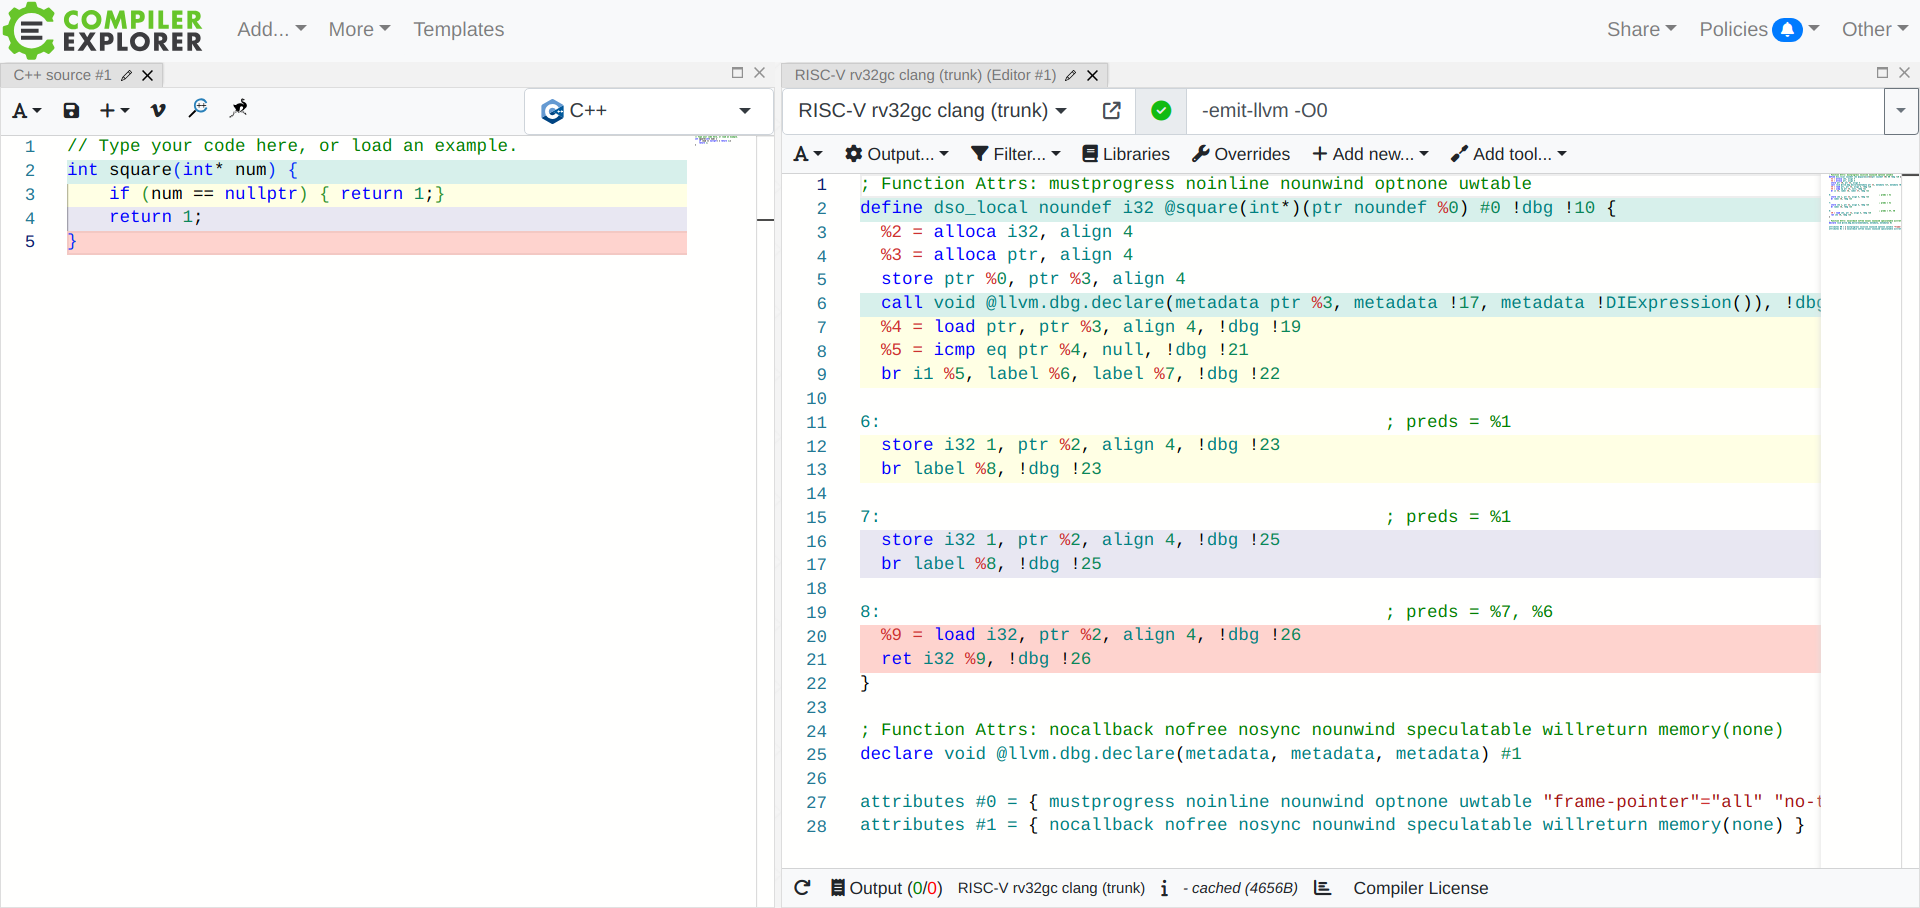
\includegraphics[scale=0.3]{image/godbolt.png}
\caption{Godbolt 使用截图}
\label{godbolt_sreenshot}
\end{figure}

图片 \ref{godbolt_sreenshot} 是一个通过在线 LLVM 环境来了解 LLVM 语言的例子。在
gofbolt 上,页面被分为两栏——左栏是你的输入,右栏是你选择的编译器在你填入的参数下的输入。下面我们将会分别介绍左右栏的使用。

左栏有一个语言选择框(位于左栏的上部)和一个代码输入框。语言选择框可以选择所使用的编程语言。

右栏上部左边部分是编译器选择框,右边部分是编译器参数框。我们此时希望将代码编译到适用于 rv32gc
平台的 LLVM 语言,而且不希望编译器做出优化(否则可能会把一部分代码直接去掉)。由于我们的编译器的目标平台是
rv32gc,且 clang 可以通过 \texttt{-emit-llvm} 来输出 LLVM 语言,因此我们在编译器选择框选择
RISCV rv32gc clang (trunk)(trunk 这里表示最新的 clang),在编译器参数框中输入 \texttt{-emit-llvm -O0}。

关于语言特性的内容,请见章节 \ref{LLVM-semantic}。

\subsubsection{本地 LLVM 环境}

你可以安装 LLVM 15 及其以上版本。截止 LLVM 17,所有的 LLVM 15 特性均可使用。

对于使用 apt 包管理的用户(debian/Ubuntu/... 用户),请参考 \href{https://apt.llvm.org/}{LLVM apt 安装文档}。

对于使用 pacman 包管理的用户,可以执行 \texttt{sudo pacman -S llvm clang} 安装最新版本的 LLVM。

你可以执行 \texttt{clang --version} 来检查 clang 是否确实安装到系统中。正常情况下,该指令会显示你的
clang 版本、目标平台等信息。

\subsection{LLVM 15 语法}\label{LLVM-semantic}

\section{从中间语言到目标代码}

\subsection{RISC-V 汇编}

\subsection{RISC-V Calling Convention}
